% questions.tex —— 2008 年·普通高等学校招生考试·上海卷·文科 · 题目内容片段（无答案）
% 由 tools/generate_projects.py 依来源总账自 2008/2008_数学真题_上海文_试题.md 生成，勿手改（改源 MD 后重跑）


状态：needs-review；依固定候选 PDF 两页（印刷页 481–482）三栏图像以 300 dpi 渲染逐题核验，图形已矢量重绘，正式构建与逐页验收待完成。源未列各题分值，不补分值。

\gkpart{一、填空题}

\begin{question}
\gkti{1}不等式 $|x-1|<1$ 的解集是\gkblank{}。

\end{question}
\begin{question}
\gkti{2}若集合 $A=\{x\mid x\leqslant2\}$，$B=\{x\mid x\geqslant a\}$ 满足 $A\cap B=\{2\}$，则实数 $a=$\gkblank{}。

\end{question}
\begin{question}
\gkti{3}若复数 $z$ 满足 $z=\mathrm i(2-z)$（$\mathrm i$ 是虚数单位），则 $z=$\gkblank{}。

\end{question}
\begin{question}
\gkti{4}若函数 $f(x)$ 的反函数为 $f^{-1}(x)=\log_2x$，则 $f(x)=$\gkblank{}。

\end{question}
\begin{question}
\gkti{5}若向量 $\boldsymbol a$，$\boldsymbol b$ 满足 $|\boldsymbol a|=1$，$|\boldsymbol b|=2$，且 $\boldsymbol a$ 与 $\boldsymbol b$ 的夹角为 $\dfrac{\pi}3$，则 $|\boldsymbol a+\boldsymbol b|=$\gkblank{}。

\end{question}
\begin{question}
\gkti{6}若直线 $ax-y+1=0$ 经过抛物线 $y^2=4x$ 的焦点，则实数 $a=$\gkblank{}。

\end{question}
\begin{question}
\gkti{7}若 $z$ 是实系数方程 $x^2+2x+p=0$ 的一个虚根，且 $|z|=2$，则 $p=$\gkblank{}。

\end{question}
\begin{question}
\gkti{8}在平面直角坐标系中，从五个点 $A(0,0)$，$B(2,0)$，$C(1,1)$，$D(0,2)$，$E(2,2)$ 中任取三个，这三点能构成三角形的概率是\gkblank{}。（结果用分数表示）

\end{question}
\begin{question}
\gkti{9}若函数 $f(x)=(x+a)(bx+2a)$（常数 $a$，$b\in\mathbf R$）是偶函数，且它的值域为 $(-\infty,4]$，则该函数的解析式 $f(x)=$\gkblank{}。

\end{question}
\begin{question}
\gkti{10}已知总体的各个体的值由小到大依次为 $2$，$3$，$3$，$7$，$a$，$b$，$12$，$13.7$，$18.3$，$20$，且总体的中位数为 $10.5$。若要使该总体的方差最小，则 $a$，$b$ 的取值分别是\gkblank{}。

\end{question}
\begin{question}
\gkti{11}在平面直角坐标系中，点 $A$，$B$，$C$ 的坐标分别为 $(0,1)$，$(4,2)$，$(2,6)$。如果 $P(x,y)$ 是 $\triangle ABC$ 围成的区域（含边界）上的点，那么当 $w=xy$ 取到最大值时，点 $P$ 的坐标是\gkblank{}。

\end{question}
\gkpart{二、选择题}

\begin{question}
\gkti{12}设 $P$ 是椭圆 $\dfrac{x^2}{25}+\dfrac{y^2}{16}=1$ 上的点。若 $F_1$，$F_2$ 是椭圆的两个焦点，则 $|PF_1|+|PF_2|$ 等于（　）

（A）$4$

（B）$5$

（C）$8$

（D）$10$

\end{question}
\begin{question}
\gkti{13}给定空间中的直线 $l$ 及平面 $\alpha$，条件“直线 $l$ 与平面 $\alpha$ 内无数条直线都垂直”是“直线 $l$ 与平面 $\alpha$ 垂直”的（　）

（A）充分非必要条件

（B）必要非充分条件

（C）充要条件

（D）既非充分又非必要条件

\end{question}
\begingroup
\renewenvironment{question}{\Needspace{0.46\textheight}}{}
\begin{question}
\gkti{14}若数列 $\{a_n\}$ 是首项为 $1$，公比为 $a-\dfrac32$ 的无穷等比数列，且 $\{a_n\}$ 各项的和为 $a$，则 $a$ 的值是（　）

（A）$1$

（B）$2$

（C）$\dfrac12$

（D）$\dfrac54$

\Needspace{0.4\textheight}
\end{question}
\endgroup
\begin{question}
\gkti{15}如图，在平面直角坐标系中，$\Omega$ 是一个与 $x$ 轴的正半轴、$y$ 轴的正半轴分别相切于点 $C$、$D$ 的定圆所围成区域（含边界），$A$、$B$、$C$、$D$ 是该圆的四等分点。若点 $P(x,y)$、点 $P'(x',y')$ 满足 $x\leqslant x'$ 且 $y\geqslant y'$，则称 $P$ 优于 $P'$。如果 $\Omega$ 中的点 $Q$ 满足：不存在 $\Omega$ 中的其它点优于 $Q$，那么所有这样的点 $Q$ 组成的集合是劣弧（　）
\nopagebreak[4]
\begin{center}% 2008 年上海卷文科第 15 题：圆 Ω 与 x、y 轴正半轴分别切于 C、D，
%   A、B、C、D 为圆的四等分点（A 上、B 右、C 下、D 左）。
% 来源 PDF：gaokaomath-src/普通高考/2008/2008上海文.pdf
% SHA-256：415d384fcd05cab11debea2d8a328f9daf1d1880ffd26c915df999f7bae589a4
% 原页：2008上海文.pdf 第 1 页（A3 三栏）第 2 栏，书页码 481。
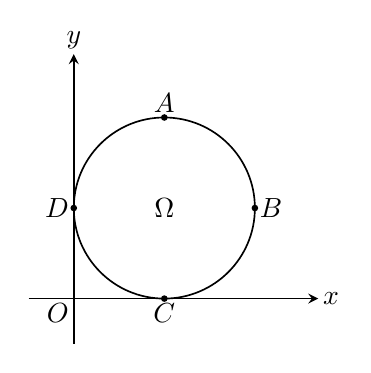
\begin{tikzpicture}[x=1.15cm, y=1.15cm, semithick,
  every node/.style={inner sep=1.5pt}]
  \draw[->,>=stealth] (-0.5,0) -- (2.7,0) node[right] {$x$};
  \draw[->,>=stealth] (0,-0.5) -- (0,2.7) node[above] {$y$};
  \node[below left] at (0,0) {$O$};
  \draw (1,1) circle (1);
  \node at (1,1) {$\Omega$};
  \fill (1,2) circle (1.2pt); \node[above] at (1,2) {$A$};
  \fill (2,1) circle (1.2pt); \node[right] at (2,1) {$B$};
  \fill (1,0) circle (1.2pt); \node[below] at (1,0) {$C$};
  \fill (0,1) circle (1.2pt); \node[left] at (0,1) {$D$};
\end{tikzpicture}
\end{center}
\nopagebreak[4]
（A）$\widehat{AB}$

（B）$\widehat{BC}$

（C）$\widehat{CD}$

（D）$\widehat{DA}$

\end{question}
\gkpart{三、解答题}

\Needspace{0.4\textheight}
\begingroup
\renewenvironment{question}{\Needspace{0.44\textheight}}{}
\begin{question}
\gkti{16}如图，在棱长为 $2$ 的正方体 $ABCD-A_1B_1C_1D_1$ 中，$E$ 是 $BC_1$ 的中点。求直线 $DE$ 与平面 $ABCD$ 所成角的大小。（结果用反三角函数表示）
\nopagebreak[4]
\begin{center}% 2008 年上海卷文科第 16 题：棱长 2 的正方体 ABCD-A1B1C1D1，E 为 BC1 的中点，
%   求直线 DE 与平面 ABCD 所成的角。
% 来源 PDF：gaokaomath-src/普通高考/2008/2008上海文.pdf
% SHA-256：415d384fcd05cab11debea2d8a328f9daf1d1880ffd26c915df999f7bae589a4
% 原页：2008上海文.pdf 第 1 页（A3 三栏）第 2 栏，书页码 481。
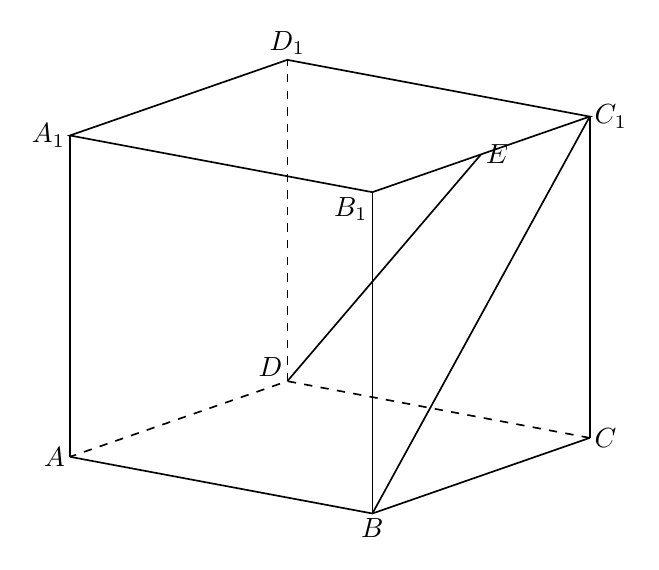
\begin{tikzpicture}[scale=1.2, semithick,
  every node/.style={inner sep=1.5pt}]
  \coordinate (A)  at (0.0,0.9);
  \coordinate (B)  at (3.2,0.3);
  \coordinate (C)  at (5.5,1.1);
  \coordinate (D)  at (2.3,1.7);
  \coordinate (A1) at (0.0,4.3);
  \coordinate (B1) at (3.2,3.7);
  \coordinate (C1) at (5.5,4.5);
  \coordinate (D1) at (2.3,5.1);
  \coordinate (E)  at (4.35,4.1);

  \draw (A) -- (B) -- (C);
  \draw[dashed] (C) -- (D) -- (A);
  \draw (A) -- (A1);
  \draw (B) -- (B1);
  \draw (C) -- (C1);
  \draw (D1) -- (A1) -- (B1) -- (C1) -- cycle;
  \draw[dashed] (D) -- (D1);

  \draw (D) -- (E);
  \draw (B) -- (C1);

  \node[left] at (A) {$A$};
  \node[below] at (B) {$B$};
  \node[right] at (C) {$C$};
  \node[above left] at (D) {$D$};
  \node[left] at (A1) {$A_1$};
  \node[below left] at (B1) {$B_1$};
  \node[right] at (C1) {$C_1$};
  \node[above] at (D1) {$D_1$};
  \node[right] at (E) {$E$};
\end{tikzpicture}
\end{center}
\nopagebreak[4]
\Needspace{0.4\textheight}
\end{question}
\endgroup
\begin{question}
\gkti{17}如图，某住宅小区的平面图呈扇形 $AOC$。小区的两个出入口设置在点 $A$ 及点 $C$ 处，小区里有两条笔直的小路 $AD$、$DC$，且拐弯处的转角为 $120^\circ$。已知某人从 $C$ 沿 $CD$ 走到 $D$ 用了 $10$ 分钟，从 $D$ 沿 $DA$ 走到 $A$ 用了 $6$ 分钟。若此人步行的速度为每分钟 $50$ 米，求该扇形的半径 $OA$ 的长。（精确到 $1$ 米）
\nopagebreak[4]
\begin{center}% 2008 年上海卷文科第 17 题：扇形 AOC，出入口在 A、C，内部小路 AD、DC，
%   拐弯处 D 的转角为 120°，CD=500 m，DA=300 m。
% 来源 PDF：gaokaomath-src/普通高考/2008/2008上海文.pdf
% SHA-256：415d384fcd05cab11debea2d8a328f9daf1d1880ffd26c915df999f7bae589a4
% 原页：2008上海文.pdf 第 1 页（A3 三栏）第 3 栏，书页码 481。
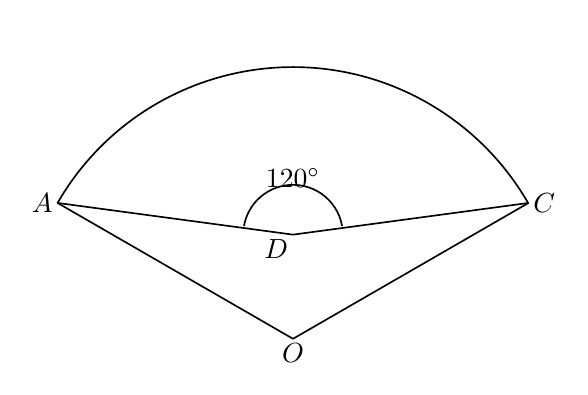
\begin{tikzpicture}[scale=1.15, semithick,
  every node/.style={inner sep=1.5pt}]
  \coordinate (O) at (0,0);
  \coordinate (A) at (-2.6,1.5);
  \coordinate (C) at (2.6,1.5);
  \coordinate (D) at (0,1.15);

  % 扇形弧
  \draw (A) arc[start angle=150, end angle=30, radius=3.0];
  \draw (O) -- (A);
  \draw (O) -- (C);

  % 小路
  \draw (A) -- (D) -- (C);

  % 转角
  \draw (D) ++(10:0.55) arc[start angle=10, end angle=170, radius=0.55];
  \node at (0,1.78) {$120^\circ$};

  \node[left] at (A) {$A$};
  \node[right] at (C) {$C$};
  \node[below left] at (D) {$D$};
  \node[below] at (O) {$O$};
\end{tikzpicture}
\end{center}
\nopagebreak[4]
\end{question}
\begin{question}
\gkti{18}已知函数 $f(x)=\sin2x$，$g(x)=\cos\left(2x+\dfrac{\pi}6\right)$，直线 $x=t$（$t\in\mathbf R$）与函数 $f(x)$、$g(x)$ 的图象分别交于 $M$、$N$ 两点。

（1）当 $t=\dfrac{\pi}4$ 时，求 $|MN|$ 的值；

（2）求 $|MN|$ 在 $t\in\left[0,\dfrac{\pi}2\right]$ 时的最大值。

\end{question}
\begin{question}
\gkti{19}已知函数 $f(x)=2^x-\dfrac1{2^{|x|}}$。

（1）若 $f(x)=2$，求 $x$ 的值；

（2）若 $2^tf(2t)+mf(t)\geqslant0$ 对于 $t\in[1,2]$ 恒成立，求实数 $m$ 的取值范围。

\end{question}
\begin{question}
\gkti{20}已知双曲线 $C:\dfrac{x^2}2-y^2=1$。

（1）求双曲线 $C$ 的渐近线方程；

（2）已知点 $M$ 的坐标为 $(0,1)$。设 $P$ 是双曲线 $C$ 上的点，$Q$ 是点 $P$ 关于原点的对称点。记 $\lambda=\overrightarrow{MP}\cdot\overrightarrow{MQ}$，求 $\lambda$ 的取值范围；

（3）已知点 $D$、$E$、$M$ 的坐标分别为 $(-2,-1)$、$(2,-1)$、$(0,1)$，$P$ 为双曲线 $C$ 上在第一象限内的点。记 $l$ 为经过原点与点 $P$ 的直线，$s$ 为 $\triangle DEM$ 截直线 $l$ 所得线段的长。试将 $s$ 表示为直线 $l$ 的斜率 $k$ 的函数。

\end{question}
\begin{question}
\gkti{21}已知数列 $\{a_n\}$：$a_1=1$，$a_2=2$，$a_3=r$，$a_{n+3}=a_n+2$（$n$ 是正整数），与数列 $\{b_n\}$：$b_1=1$，$b_2=0$，$b_3=-1$，$b_4=0$，$b_{n+4}=b_n$（$n$ 是正整数）。记 $T_n=b_1a_1+b_2a_2+b_3a_3+\cdots+b_na_n$。

（1）若 $a_1+a_2+a_3+\cdots+a_{12}=64$，求 $r$ 的值；

（2）求证：当 $n$ 是正整数时，$T_{12n}=-4n$；

（3）已知 $r>0$，且存在正整数 $m$，使得在 $T_{12m+1}$，$T_{12m+2}$，$\cdots$，$T_{12m+12}$ 中有 $4$ 项为 $100$，求 $r$ 的值，并指出哪 $4$ 项为 $100$。

\end{question}